\textbf{PDP (Partial Dependence Plot, график частичной зависимости)} -- график, который показывает зависимость прогноза модели от значения отдельного признака. С его помощью мы можем понять, как некоторый признак влияет на предсказание. Данный график можно изобразить для двух либо трех признаков из имеющихся.

\subsubsection{Идея}
Визуализация -- это отличный способ интерпретации. Если мы хотим понять, как признаки влияют на результат, можно посмотреть, как меняется прогноз от изменения одного признака при прочих равных. В идеальной ситуации мы бы построили график зависимости результата от всех признаков и меняли бы только один. Однако мы сталкиваемся с проблемой: если признаков больше двух, построить график не получится. Поэтому чтобы сохранить возможность визуализации, можно анализировать зависимость результата от одного признака без учета влияния остальных, построив график зависимости от одного признака. Аналогично можно изучать влияние одновременно двух признаков, построив трехмерный график.

\underline{Пример PDP для одного признака}
\vspace{-7mm}

\begin{figure}[h]
	\centering{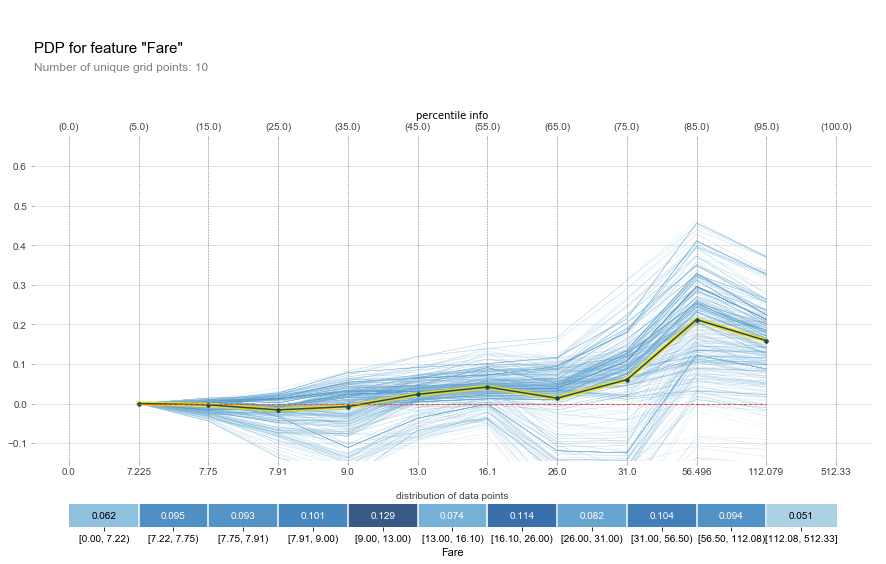
\includegraphics[width=0.95\linewidth]{pics/pdp1.png}}
\end{figure}

Желтая линия показывает, как в среднем выбранный признак <<Fare>> влияет на предсказание. Для упрощения визуализации значения признака по всем объектам были разбиты по квантилям -- так график для непрерывного признака становится более наглядным. По оси ординат указан непосредственно эффект признака: значение <<-0.1>> указывает на то, что признак уменьшает итоговое предсказание на 0.1. То есть данный график показывает <<предельный эффект>> признака. В данном случае можно сделать вывод, что <<Fare>> незначительно влияет при маленьких значениях признака. Но при возрастании начинает вносить ощутимый вклад в предсказание -- и зависимость при этом скорее положительная, но нелинейная.

\underline{Примеры PDP для двух признаков}
\vspace{-3mm}

\begin{figure}[h]
	\centering{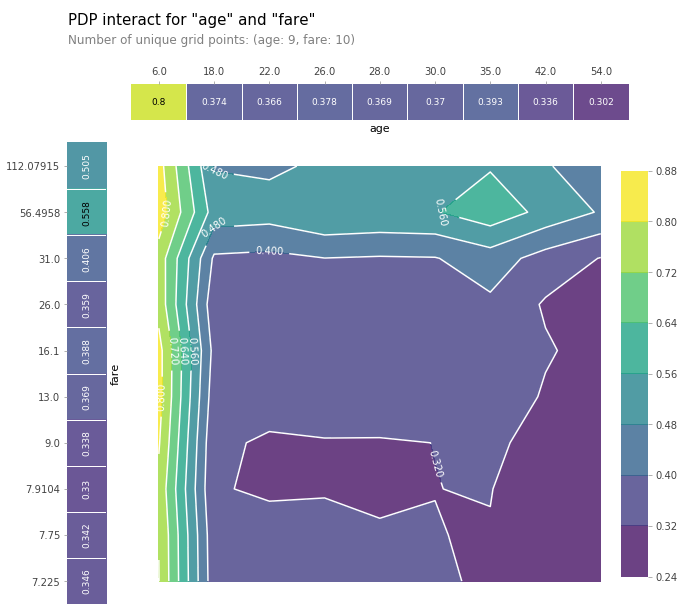
\includegraphics[width=0.75\linewidth]{pics/pdp2.png}}
\end{figure}
\vspace{-5mm}
\begin{figure}[h!]
	\centering{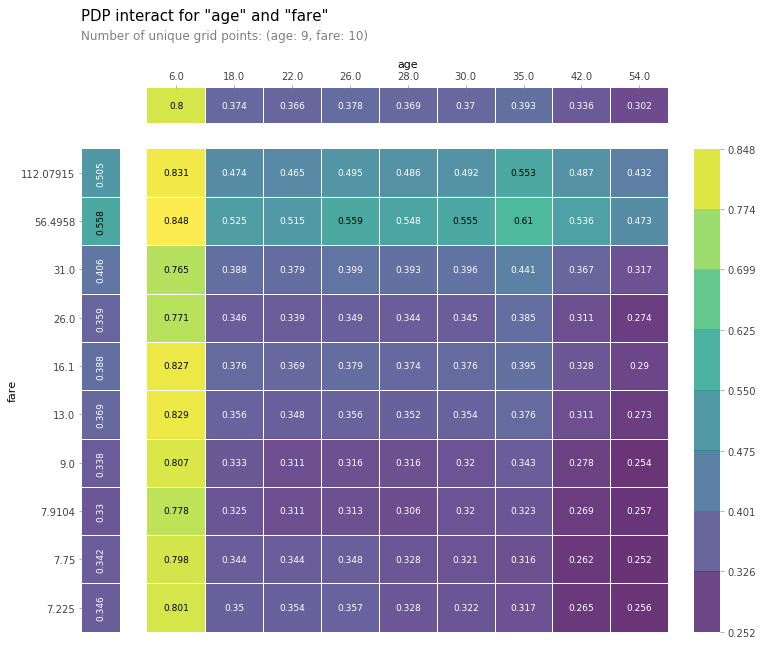
\includegraphics[width=0.76\linewidth]{pics/pdp3.png}}
\end{figure}

Отличие данных графиков от предыдущего заключается в том, что он показывает не предельные эффекты, а непосредственно предсказания модели. Первый график показывает линии уровня получившейся функции двух аргументов. Второй -- упрощенное представление линий уровня в виде сетки. Шкалы над и слева от графика показывают влияние каждого признака по отдельности -- сжатое представление графика для одного признака. По обоим графикам видно, что наименьшее значение предсказания достигается, когда значение <<fare>> наименьшее, а <<age>> -- наибольшее. Также можно отметить экстремум функции, который достигается при <<fare>> $\approx 56.4958$ и <<age>> $\approx 35$ -- зависимость нелинейная от обоих аргументов.